\documentclass[a4paper, 11pt]{article}
\usepackage[margin=2cm]{geometry}
\usepackage{xcolor}
\usepackage{graphicx}
\newcommand{\useicon}[2][8pt]{\includegraphics[height=#1]{./icons/#2.png}}
\usepackage{amssymb}

\usepackage{tabularx}
\usepackage{hyperref}
\hypersetup{
    pdftitle={Candidature a la Qualification aux Fonctions de Maitre de Conferences},
    bookmarks=true
}
\newcommand{\mailto}[2]{\href{mailto:#2}{\color{blue}{#1}~\useicon{mail}}}
\newcommand{\linkto}[2]{\href{#2}{\color{purple}{#1}~\useicon{link}}}
\newcommand{\jumpto}[2]{\hyperref[#2]{\color{cyan!70!black}{#1}~\useicon{jump}}}

\setlength{\parindent}{0pt}
\setlength{\tabcolsep}{1mm}
\hyphenpenalty=10000

\begin{document}
    \title{Candidature {\`a} la Qualification \\
           aux Fonctions de Ma{\^i}tre de Conf{\'e}rences \\
           -- Curriculum Vit{\ae} --}
    \author{Guillaume Bono}
    \date{Novembre 2020}

    \maketitle
    
    \section*{Identit{\'e}}

    \noindent
    \begin{minipage}{.09\textwidth}
        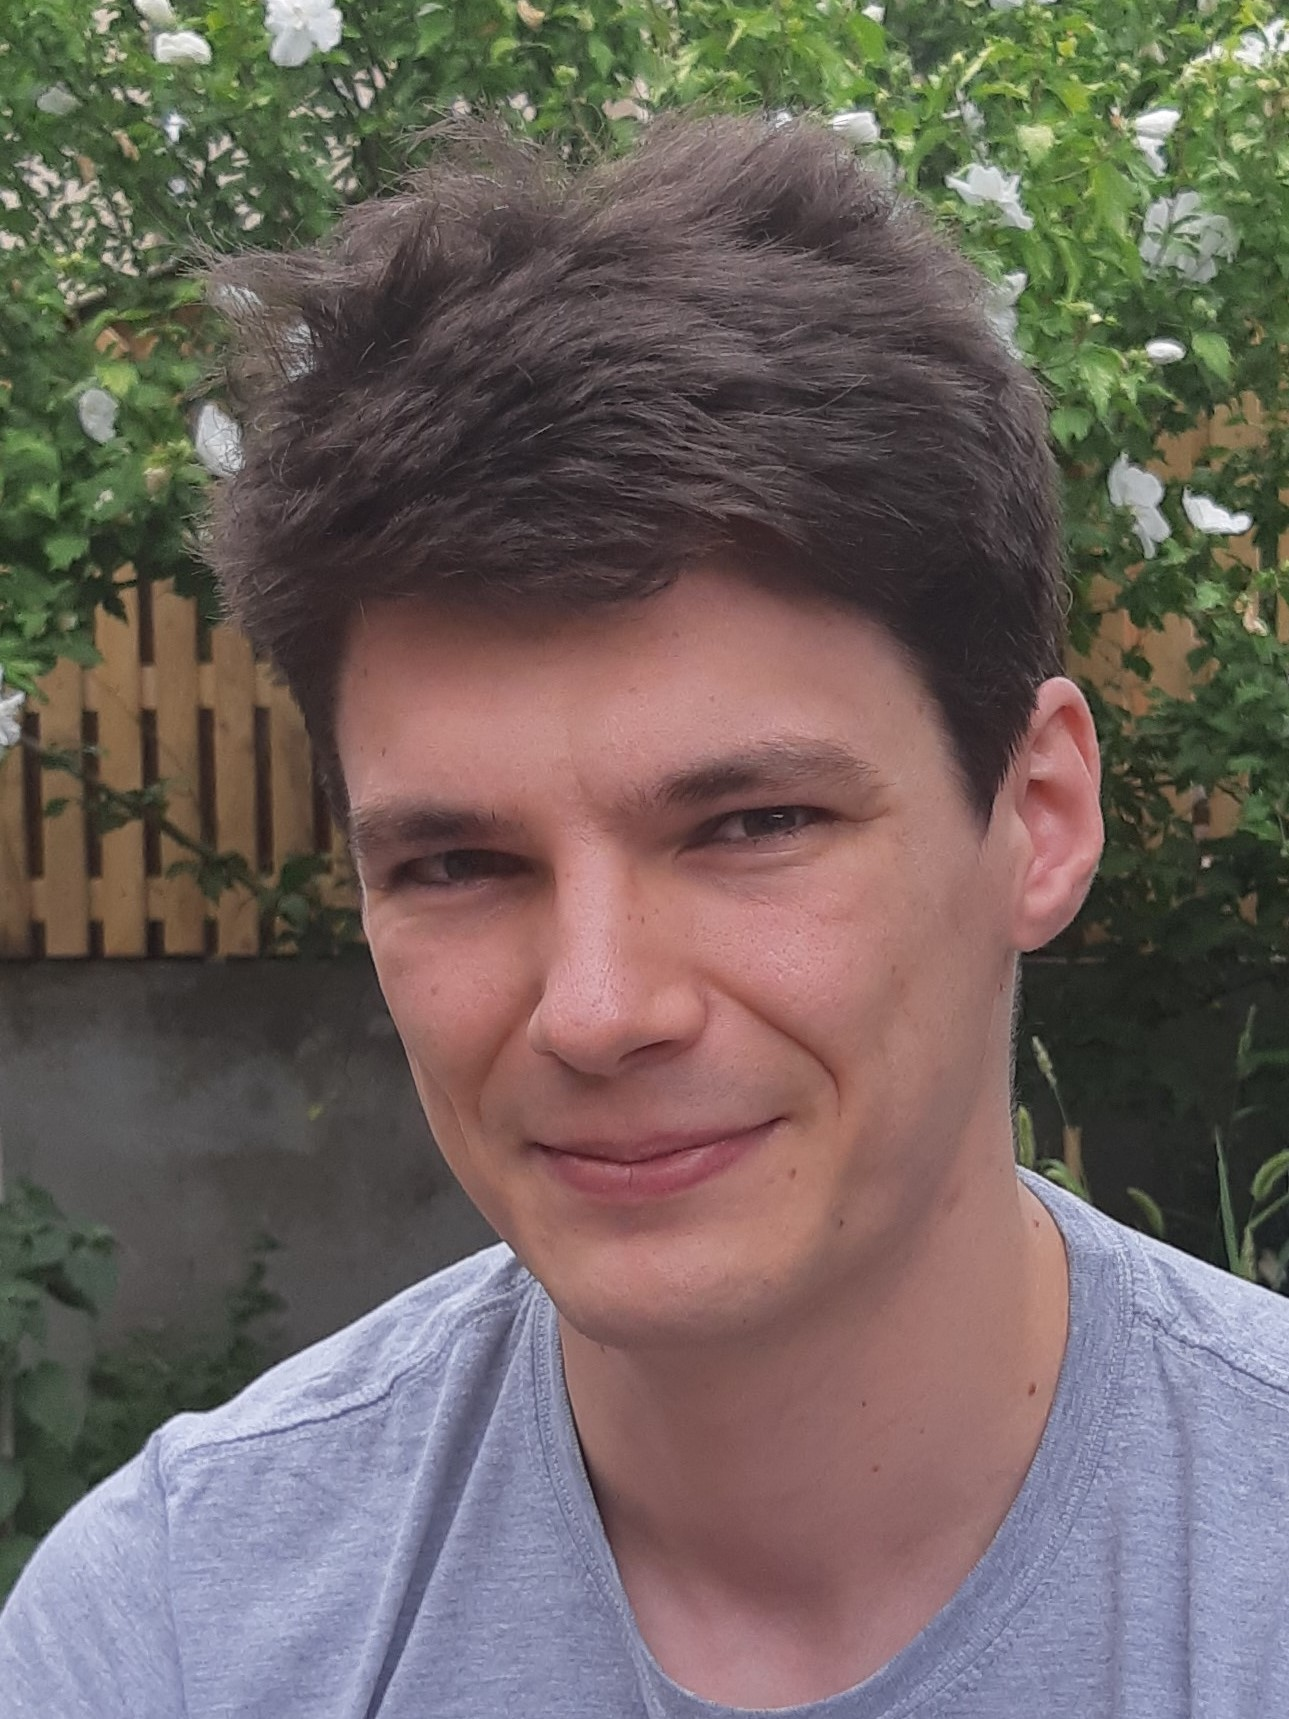
\includegraphics[width=\textwidth]{./photo_gbo_bio.jpg}
    \end{minipage}
    \begin{minipage}{.44\textwidth}
        \fcolorbox{black}{blue!10}{
            \begin{tabular}{>{\small}r c l}
                Nom               &: &\bf Bono \\
                Pr{\'e}nom        &: &\bf Guillaume \\
                \hline
                Date de naissance &: &22 Novembre 1992 \\
                Lieu de naissance &: &Bron, Rh{\^o}ne, France \\
                Nationalit{\'e}   &: &Fran{\c c}aise \\
            \end{tabular}
        }
    \end{minipage}
    \begin{minipage}{.46\textwidth}
        \colorbox{yellow!10}{
            \begin{tabular}{>{\small}r c l}
                Adresse           &: &22 rue Th{\'e}nard \\
                                  &  &69008, Lyon, France \\
                T{\'e}l{\'e}phone &: &+33 6 85 07 97 05 \\
                Courriel          &: &\mailto{bono.guillaume@gmail.com}{bono.guillaume@gmail.com} \\
            \end{tabular}
        }
    \end{minipage}

    \section*{\useicon[12pt]{edu}~Parcours Universitaire}

    \colorbox{yellow!30}{
        \begin{tabularx}{.97\textwidth}{>{\raggedleft\small}p{.18\textwidth} c X}
            Intitul{\'e}           &: &\bf Doctorat de l'Universit{\'e} de Lyon op{\'e}r{\'e} au sein de l'INSA Lyon \\
            {\'E}tablissement      &: &\linkto{INSA Lyon}{https://www.insa-lyon.fr} \\
            Lieu                   &: &Villeurbanne, Rh{\^o}ne, France \\
            Date                   &: &Octobre 2020 \\
            Titre                  &: &Apprentissage par Renforcement Multi-Agents Profond pour les \\
                                   &  &Probl{\`e}mes de Planification de Tourn{\'e}es Dynamiques et Stochastiques \\
            Sp{\'e}cialit{\'e}     &: &Informatique (Intelligence Artificielle / Recherche Op{\'e}rationnelle) \\
            Rattachement           &: &INSA Lyon, INRIA, Laboratoire \linkto{CITI}{http://www.citi-lab.fr}, {\'E}quipe \linkto{CHROMA}{https://team.inria.fr/chroma} \\
            \hline
            Directeur              &: &\mailto{Olivier Simonin}{olivier.simonin@insa-lyon.fr} (INSA Lyon, INRIA, CITI, CHROMA) \\
            Co-encadrants          &: &\mailto{Jilles Dibangoyes}{jilles-steeve.dibangoye@insa-lyon.fr} (INSA Lyon, INRIA, CITI, CHROMA) \\
                                   &  &\mailto{La{\"e}titia Matignon}{florian.pereyron@volvo.com} (Universit{\'e} Lyon 1, CNRS, LIRIS) \\
                                   &  &\mailto{Florian Pereyron}{florian.pereyron@volvo.com} (Volvo group, Advanced Tech. and Research) \\
            \hline
            Pr{\'e}sident du jury  &: &Ren{\'e} Mandiau (UPFH, CNRS, LAMIH) \\
            Rapporteurs            &: &Fran{\c c}ois Charpillet (INRIA, LORIA) \\
                                   &  &Romain Billot (IMT Atlantique, CNRS, Lab-STICC) \\
            Examinateurs           &: &Aur{\'e}lie Beynier (Sorbonne Universit{\'e}, CNRS, LIP6) \\
                                   &  &Christian Wolf (INSA Lyon, CNRS, LIRIS) \\
        \end{tabularx}
    }

    \vspace{5mm}
    \colorbox{yellow!10}{
        \begin{tabularx}{.97\textwidth}{>{\raggedleft\small}p{.18\textwidth} c X}
            Intitul{\'e}           &: &\bf Master of Science in Computer Science \\
            {\'E}tablissement      &: &\linkto{Georgia Institute of Technology}{https://www.gatech.edu} \\
            Lieux                  &: &Atlanta, GA, USA \\
                                   &  &Metz, Lorraine, France \\
            Date                   &: &Mai 2016 \\
        \end{tabularx}
    }

    \vspace{5mm}
    \colorbox{yellow!10}{
        \begin{tabularx}{.97\textwidth}{>{\raggedleft\small}p{.18\textwidth} c X}
            Intitul{\'e}           &: &\bf Dipl{\^o}me d'Ing{\'e}nieur de l'{\'E}cole Sup{\'e}rieure d'{\'E}lectricit{\'e} \\
            {\'E}tablissement      &: &\linkto{CentraleSup{\'e}lec}{https://www.centralesupelec.fr} \\
            Lieux                  &: &Gif-sur-Yvette, Essone, France \\
                                   &  &Metz, Lorraine, France \\
            Date                   &: &F{\'e}vrier 2016 \\
            \hline
            Projet Fin d'{\'E}tude &: &Conception (m{\'e}ca. et  {\'e}lec.) et programmation d'une barge autonome \\
                                   &  &sur base Android pour la surveillance du d{\'e}veloppement algal \\
            Encadrant              &: &\mailto{C{\'e}dric Pradalier}{cedric.pradalier@gatech.edu} (GATech Lorraine, CNRS, DREAM) \\
            Soci{\'e}t{\'e}        &: &\linkto{Sofchem}{http://www.sofchem.fr} \\
            \hline
            Stage Fin d'{\'E}tude  &: &Int{\'e}gration et r{\'e}-entra{\^i}nement d'un r{\'e}seau de neurones profond ``ModDrop'' \\
                                   &  &pour la reconnaissance de gestes sur une carte nVidia Tegra K1 \\
            Responsable            &: &\mailto{Florian Nebout}{florian.nebout@awabot.com} (Awabot) \\
            Soci{\'e}t{\'e}        &: &\linkto{Awabot}{https://awabot.com} \\
        \end{tabularx}
    }

    \section*{\useicon[12pt]{work}~Exp{\'e}riences Professionnelles}

    \colorbox{yellow!30}{
        \begin{tabularx}{.97\textwidth}{>{\raggedleft\small}p{.18\textwidth} c X}
            Intitul{\'e}      &: &\bf Ing{\'e}nieur de Recherche \\
            Dates             &: &de Novembre 2020 {\`a} aujourd'hui \\
            {\'E}tablissement &: &\linkto{INSA Lyon}{https://www.insa-lyon.fr} \\
            Statut            &: &CDD \\
            Description       &: &Transfert de politiques de navigation de la simulation au monde r{\'e}el --
                Apprentissage -- R{\'e}seaux de neurones profonds -- Robots mobiles \\
        \end{tabularx}
    }

    \vspace{3mm}
    \colorbox{yellow!10}{
        \begin{tabularx}{.97\textwidth}{>{\raggedleft\small}p{.18\textwidth} c X}
            Intitul{\'e}      &: &\bf Attach{\'e} Temporaire d'Enseignement et de Recherche \\
            Dates             &: &d'Octobre 2019 {\`a} Septembre 2020 \\
            {\'E}tablissement &: &\linkto{INSA Lyon}{https://www.insa-lyon.fr} \\
            Statut            &: &CDD \\
            Description       &: &Poursuite travaux de th{\`e}se -- Enseignement info. et r{\'e}seau, d{\'e}partement TC \\
                &  &(c.f. \jumpto{Activit{\'e}s d'Enseignement}{sec:teach}) \\
        \end{tabularx}
    }

    \vspace{3mm}
    \colorbox{yellow!10}{
        \begin{tabularx}{.97\textwidth}{>{\raggedleft\small}p{.18\textwidth} c X}
            Intitul{\'e}      &: &\bf Doctorant \\
            Dates             &: &d'Octobre 2016 {\`a} Septembre 2019 \\
            {\'E}tablissement &: &\linkto{INSA Lyon}{https://www.insa-lyon.fr} \\
            Statut            &: &CDD \\
            Description       &: &Apprentissage par renforcement profond pour la planification de tourn{\'e}es \\
                              &  &(c.f. \jumpto{Activit{\'e}s de Recherche}{sec:research}) \\
        \end{tabularx}
    }

    \vspace{3mm}
    \colorbox{yellow!10}{
        \begin{tabularx}{.97\textwidth}{>{\raggedleft\small}p{.18\textwidth} c X}
            Intitul{\'e}      &: &\bf Ing{\'e}nieur R\&D \\
            Dates             &: &d'Octobre 2015 {\`a} D{\'e}cembre 2015 \\
            Soci{\'e}t{\'e}   &: &\linkto{Awabot}{https://awabot.com} \\
            Statut            &: &CDD \\
            Description       &: &Poursuite des travaux de stage : Impl{\'e}m. reco. gestes via DNN -- Collecte donn{\'e}es d'entra{\^i}nement
                -- Segmentation profondeur -- Gestion projet \\
        \end{tabularx}
    }

    \section*{\useicon[12pt]{perso}~Exp{\'e}rience Personnelle}

    \colorbox{yellow!10}{
        \begin{tabularx}{.97\textwidth}{>{\raggedleft\small}p{.18\textwidth} c X}
            Intitul{\'e}      &: &\bf Technicien son et lumi{\`e}re, Responsable ``son'' \\
            Dates             &: &d'Octobre 2012 {\`a} Ao{\^u}t 2014 \\
            Association       &: &\linkto{Sono Sup{\'e}lec}{https://www.sbcs-events.fr} \\
            Statut            &: &B{\'e}n{\'e}vol \\
            Description       &: &Installation structure, son et lumi{\`e}re -- Animation DJ -- R{\'e}gie Concert --
                Logistique -- Entretien mat{\'e}riel -- Formation nouveaux membres \\
        \end{tabularx}
    }

    \section*{\useicon[12pt]{teach}~Activit{\'e}s d'Enseignement}
    \label{sec:teach}

    \colorbox{green!10}{\parbox{.98\textwidth}{
        \small\itshape
        \hspace{7mm}J'ai men{\'e} l'ensemble de mes activit{\'e}s d'enseignement au sein du d{\'e}partement T{\'e}l{\'e}communication (TC) de l'{\bf INSA Lyon}.
        Je m'adressais donc {\`a} des {\bf {\'e}l{\`e}ves ing{\'e}nieurs} de niveaux {\'e}quivalents {\bf L3 {\`a} M2}.
        Cette section liste et d{\'e}taille le contenu de chaque cours dont j'ai particip{\'e} {\`a} l'encadrement,
        ainsi que mon implication dans chacun d'eux.
    }}

    \subsection*{R{\'e}capitulatif des heures d'enseignement dispens{\'e}es}
    \colorbox{yellow!30}{
        \begin{tabularx}{.97\textwidth}{c c c r >{\small}X c c c}
            \small Statut &\small Ann{\'e}e &\small Niveau & &\small Intitul{\'e} &\small Volume &\small Nature \\
            \hline
            vacataire &2018-19 &L3        &PIT  &- Passeport Informatique T{\'e}l{\'e}com             &24h &TD \\
            ATER      &2019-20 &L3        &PIT  &- Passeport Informatique T{\'e}l{\'e}com             &24h &TD \\
            ATER      &2019-20 &L3        &PPC  &- Programmation Parall{\`e}le et Concurrente         &22h &TD, projets \\
            ATER      &2019-20 &L3        &WEB  &- Programmation WEB dynamique                        &34h &TD, projets \\
            ATER      &2019-20 &L3        &CRO  &- C language and programming ROots                   &18h &TP \\
            ATER      &2019-20 &L3        &MAC  &- M{\'e}canismes d'Acc{\`e}s au Canal                &16h &TD, TP \\
            ATER      &2019-20 &L3        &IP   &- Protocoles TCP/IP                                  &10h &TP \\
            ATER      &2019-20 &L3 (intl) &DBM2 &- DataBase Management 2                              &20h &TD-cours \\
            ATER      &2019-20 &M1        &IAT  &- Intelligence Artificielle pour les T{\'e}l{\'e}com &6h  &TD \\
            vacataire &2018-19 &M2        &SMR  &- Syst{\`e}mes Multi-Robots                          &12h &TP, projets \\
            ATER      &2019-20 &M2        &SMR  &- Syst{\`e}mes Multi-Robots                          &10h &TP, projets \\
            ATER      &2019-20 &M2        &CSAD &- Calcul Scientifique et Analyse de Donn{\'e}es      &6h  &TD-cours \\
            \hline
                      &        &          &     &\bf Total                                            &\bf 202h \\
        \end{tabularx}
    }

    \subsection*{PIT - Passeport Informatique T{\'e}l{\'e}com}
    \begin{minipage}[t]{.54\textwidth}
        \small
        Ces TDs sont parmi les premi{\`e}res heures que les {\'e}l{\`e}ves ont en entrant au d{\'e}partement.
        L'objectif est de les familiariser avec les outils dont ils auront besoin par la suite,
        principalement la ligne de commande (\texttt{bash}) et la programmation (\texttt{python}).
        J'ai encadr{\'e} plusieurs groupes de TD, avec un suivi des {\'e}l{\`e}ves au cas par cas,
        et des interventions pour tous sur des points de difficult{\'e} redondants.
        J'ai aussi d{\'e}velopp{\'e} un squelette de code {\`a} compl{\'e}ter par les {\'e}l{\`e}ves avec tests unitaires automatiques
        pour le projet final de ce module (\linkto{r{\'e}solution de sudoku}{https://gitlab.inria.fr/gbono/pit-sudoku}).
    \end{minipage}
    \begin{minipage}[t]{.44\textwidth}
        \colorbox{yellow!10}{\begin{tabularx}{.97\textwidth}[t]{>{\small}r c X}
            Responsable &: &\mailto{Jilles Dibangoye}{jilles-steeve.dibangoye@insa-lyon.fr} \\
            Ann{\'e}es  &: &2018-19 et 2019-20 \\
            Niveau      &: &3TC (L3) \\
            Volume      &: &2$\times$ 24h \\
            Nature      &: &TD \\
        \end{tabularx}}
    \end{minipage}
    
    \subsection*{PPC - Programmation Parall{\`e}le et Concurrente}
    \begin{minipage}[t]{.54\textwidth}
        \small
        Ce cours vise {\`a} introduire aux {\'e}l{\`e}ves les concepts et probl{\'e}matiques de la programmation concurrente,
        incluant la synchronisation de fils d'ex{\'e}cution et le partage de ressource.
        J'ai encadr{\'e} un groupe de TD (avec support existant, en \texttt{python}),
        et l'ai accompagn{\'e} lors du projet final de ce module (un jeu de carte multi-joueur simultan{\'e})
        dont j'ai particip{\'e} {\`a} la d{\'e}finition du sujet.
    \end{minipage}
    \begin{minipage}[t]{.44\textwidth}
        \colorbox{yellow!10}{\begin{tabularx}{.97\textwidth}[t]{>{\small}r c X}
            Responsable &: &\mailto{Razmig Kechichian}{razmig.kechichian@insa-lyon.fr} \\
            Ann{\'e}e   &: &2019-20 \\
            Niveau      &: &3TC (L3) \\
            Volume      &: &22h \\
            Nature      &: &TD, projets \\
        \end{tabularx}}
    \end{minipage}
    
    \subsection*{WEB - Programmation WEB dynamique}
    \begin{minipage}[t]{.54\textwidth}
        \small
        Ce cours apprend aux {\'e}l{\`e}ves {\`a} cr{\'e}er un site web moderne.
        Nous les avons organis{\'e} en groupes de travail,
        chacun charg{\'e} de mener {\`a} terme un projet.
        Ils avaient {\`a} g{\'e}rer eux m{\^e}me leur projet avec des outils de version (\texttt{git}) et de suivi (mindmap, \texttt{github}),
        faire des choix technologiques (par ex. \texttt{angular}, \texttt{express} et \texttt{mongodb}), et se r{\'e}partir le travail (frontend, backend, stockage).
        L'objectif {\'e}tait d'aboutir {\`a} un site web fonctionnel, fiable et durable,
        avec une sensibilisation au devops.
    \end{minipage}
    \begin{minipage}[t]{.44\textwidth}
        \colorbox{yellow!10}{\begin{tabularx}{.97\textwidth}[t]{>{\small}r c X}
            Responsable &: &\mailto{Pierre Fran{\c c}ois}{pierre.francois@insa-lyon.fr} \\
            Ann{\'e}e   &: &2019-20 \\
            Niveau      &: &3TC (L3) \\
            Volume      &: &34h \\
            Nature      &: &TD, projets \\
        \end{tabularx}}
    \end{minipage}
    
    \subsection*{CRO - C language and programming ROots}
    \begin{minipage}[t]{.54\textwidth}
        \small
        Ce cours vise {\`a} initier les {\'e}l{\`e}ves aux fondements de l'informatique par l'interm{\'e}diaire du langage C,
        avec des concepts comme la compilation, les pointeurs et l'organisation de la m{\'e}moire, en tendant vers de l'embarqu{\'e}.
        J'ai encadr{\'e} plusieurs groupes de TP, en aidant les {\'e}l{\`e}ves au cas par cas,
        et j'ai propos{\'e} des corrections alternatives aux diff{\'e}rents sujets (supports existants).
    \end{minipage}
    \begin{minipage}[t]{.44\textwidth}
        \colorbox{yellow!10}{\begin{tabularx}{.97\textwidth}[t]{>{\small}r c X}
            Responsable &: &\mailto{Tanguy Risset}{tanguy.risset@insa-lyon.fr} \\
            Ann{\'e}e   &: &2019-20 \\
            Niveau      &: &3TC (L3) \\
            Volume      &: &18h \\
            Nature      &: &TP \\
        \end{tabularx}}
    \end{minipage}
    
    \subsection*{MAC - M{\'e}canismes d'Acc{\`e}s au Canal}
    \begin{minipage}[t]{.54\textwidth}
        \small
        Ce cours apprend aux {\'e}l{\`e}ves le fonctionnement de la couche 2 (MAC) des mod{\`e}les OSI et TCP/IP.
        J'ai dirig{\'e} un groupe de TD pou r{\'e}soudre des exercices traitant des probl{\`e}mes d'acc{\`e}s au canal (ethernet, wifi, \dots).
        J'ai aussi encadr{\'e} un groupe de TP dans lequel les {\'e}l{\`e}ves manipulent de l'{\'e}quipement professionnel (switchs, etc\dots).
    \end{minipage}
    \begin{minipage}[t]{.44\textwidth}
        \colorbox{yellow!10}{\begin{tabularx}{.97\textwidth}[t]{>{\small}r c X}
            Responsable &: &\mailto{Fabrice Valois}{fabrice.valois@insa-lyon.fr} \\
            Ann{\'e}e   &: &2019-20 \\
            Niveau      &: &3TC (L3) \\
            Volume      &: &16h \\
            Nature      &: &TD, TP \\
        \end{tabularx}}
    \end{minipage}
    
    \subsection*{IP - Protocoles TCP/IP}
    \begin{minipage}[t]{.54\textwidth}
        \small
        Ce cours apprend aux {\'e}l{\`e}ves le fonctionnement de la couche 3 (IP) des mod{\`e}les OSI et TCP/IP.
        J'ai encadr{\'e} des groupes de TP dans lesquels les {\'e}l{\`e}ves manipulent de l'{\'e}quipement professionnel (switchs, routeurs, etc\dots).
    \end{minipage}
    \begin{minipage}[t]{.44\textwidth}
        \centering
        \colorbox{yellow!10}{\begin{tabularx}{.97\textwidth}[t]{>{\small}r c X}
            Responsable &: &\mailto{Fabrice Valois}{fabrice.valois@insa-lyon.fr} \\
            Ann{\'e}e   &: &2019-20 \\
            Niveau      &: &3TC (L3) \\
            Volume      &: &10h \\
            Nature      &: &TP \\
        \end{tabularx}}
    \end{minipage}
    
    \subsection*{DBM2 - DataBase Management 2}
    \begin{minipage}[t]{.54\textwidth}
        \small
        Ce cours de fouille de donn{\'e}es s'adresse {\`a} des {\'e}tudiants internationaux.
        Sur base de supports existants, je leur ai fait d{\'e}couvrir les bases de la fouille de donn{\'e}es,
        incluant entre autre l'importance du pr{\'e}traitement et de la visualisation des donn{\'e}es,
        la classification (par ex. arbres de d{\'e}cision), la r{\'e}gression et le partitionnement (par ex. k-mean).
        Les s{\'e}ances alternaient entre pr{\'e}sentations et exp{\'e}rimentations sur l'outil \texttt{KNIME},
        et se sont conclues sur des projets choisis par les {\'e}l{\`e}ves en se basant sur des bases de donn{\'e}es existantes
        (souvent selectionn{\'e}es sur \texttt{kaggle}).
    \end{minipage}
    \begin{minipage}[t]{.44\textwidth}
        \colorbox{yellow!10}{\begin{tabularx}{.97\textwidth}[t]{>{\small}r c X}
            Responsable &: &\mailto{Fr{\'e}d{\'e}ric Le Mou{\"e}l}{frederic.le-mouel@insa-lyon.fr} \\
            Ann{\'e}e   &: &2019-20 \\
            Niveau      &: &IST (L3 intl) \\
            Volume      &: &20h \\
            Nature      &: &TD-cours \\
        \end{tabularx}}
    \end{minipage}
    
    \subsection*{IAT - Intelligence Artificielle pour les T{\'e}l{\'e}com}
    \begin{minipage}[t]{.54\textwidth}
        \small
        Ce cours se d{\'e}compose en plusieurs sous-modules.
        Celui auquel j'ai particip{\'e} vise {\`a} apprendre aux {\'e}l{\`e}ves les bases de l'apprentissage par renforcement.
        J'ai impl{\'e}ment{\'e} un sc{\'e}nario de robot nettoyage sur une grille (gridworld)
        {\`a} partir duquel les {\'e}l{\`e}ves devaient r{\'e}impl{\'e}menter plusieurs algorithmes d'apprentissage
        comme \texttt{Q-learning} ou \texttt{Policy Gradient} et leur variante ``Deep'' avec des r{\'e}seaux de neurones (en utilisant \texttt{pytorch}).
    \end{minipage}
    \begin{minipage}[t]{.44\textwidth}
        \colorbox{yellow!10}{\begin{tabularx}{.97\textwidth}[t]{>{\small}r c X}
            Responsable &: &\mailto{Jilles Dibangoye}{jilles-steeve.dibangoye@insa-lyon.fr} \\
            Ann{\'e}e   &: &2019-20 \\
            Niveau      &: &4TC (M1) \\
            Volume      &: &6h \\
            Nature      &: &TD \\
        \end{tabularx}}
    \end{minipage}
    
    \subsection*{SMR - Syst{\`e}mes Multi-Robots}
    \begin{minipage}[t]{.54\textwidth}
        \small
        Dans ce cours, les {\'e}l{\`e}ves apprennent les bases de la robotique (perception, navigation, planification, \dots).
        J'ai particip{\'e} {\`a} l'encadrement de plusieurs TPs dans lesquels ils ont pris en main le cadre logiciel \texttt{ROS},
        impl{\'e}ment{\'e} diff{\'e}rent n{\oe}uds de navigation ({\'e}vitement d'obstacles, cartographie, \dots),
        mais aussi une application android ``t{\'e}l{\'e}commande'' pour un Turtlebot.
        J'ai aussi particip{\'e} {\`a} l'encadrement de projets sur diff{\'e}rentes plateformes robotiques (Pepper, Turtlebot, drone Parrot, \dots).
    \end{minipage}
    \begin{minipage}[t]{.44\textwidth}
        \colorbox{yellow!10}{\begin{tabularx}{.97\textwidth}[t]{>{\small}r c X}
            Responsable &: &\mailto{Olivier Simonin}{olivier.simonin@insa-lyon.fr} \\
            Ann{\'e}es  &: &2018-2019 et 2019-20 \\
            Niveau      &: &5TC (M2) \\
            Volume      &: &12h $+$ 10h \\
            Nature      &: &TP, projets \\
        \end{tabularx}}
    \end{minipage}
    
    \subsection*{CSAD - Calcul Scientifique et Analyse de Donn{\'e}es}
    \begin{minipage}[t]{.54\textwidth}
        \small
        Ce cours se d{\'e}compose en plusieurs sous-modules.
        J'ai {\'e}t{\'e} charg{\'e} de dispenser celui traitant de la th{\'e}orie des r{\'e}seaux,
        en me basant sur le livre \emph{Network Science} de A-L. Barab{\'a}zi.
        Les s{\'e}ances alternaient entre pr{\'e}sentation des concepts (graphes al{\'e}atoires, loi puissance, ph{\'e}nom{\`e}ne de petit monde, \dots)
        et prise en main en \texttt{python} avec le paquet \texttt{networkx}.
    \end{minipage}
    \begin{minipage}[t]{.44\textwidth}
        \colorbox{yellow!10}{\begin{tabularx}{.97\textwidth}[t]{>{\small}r c X}
            Responsable &: &\mailto{Razmig Kechichian}{razmig.kechichian@insa-lyon.fr} \\
            Ann{\'e}e   &: &2019-20 \\
            Niveau      &: &5TC (M2) \\
            Volume      &: &6h \\
            Nature      &: &TD-cours \\
        \end{tabularx}}
    \end{minipage} 

    \section*{\useicon[12pt]{research}~Activit{\'e}s de Recherche}
    \label{sec:research}

    \colorbox{green!10}{\parbox{.98\textwidth}{
        \small\itshape
        \hspace{7mm}La poursuite de mon doctorat, portant sur le sujet de la planification de tourn{\'e}es de v{\'e}hicules (VRP)
        dans un contexte multi-agent dynamique et stochastique, constitue ma principale activit{\'e} de recherche.
        Au cours de ces travaux, nous nous sommes pench{\'e}s sur l'application des m{\'e}thodes d'apprentissage par renforcement (RL)
        -- et en particulier l'apprentissage par renforcement profond (Deep RL) -- dans le contexte du VRP.
        Cette section r{\'e}sume les diff{\'e}rentes contributions de ma th{\`e}se, en commencant par une liste de mes publications,
        puis en revenant sur chacune d'entre elle afin d'en d{\'e}tailler le contenu.
    }}

    \subsection*{Liste de publications}

    \subsubsection*{Revue internationale avec comit{\'e} de lecture}
    \colorbox{yellow!30}{
        \begin{tabularx}{.97\textwidth}{>{\raggedleft\small}p{.18\textwidth} c X}
            Titre       &: &``Solving Multi-Agent Routing Problems using Deep Attention Mechanisms'' \\
            Auteurs     &: &G. Bono, J. Dibangoye, O. Simonin, L. Matignon, F. Pereyron \\
            Revue       &: &IEEE Transactions on Intelligent Transportation Systems \\
            Date        &: &Juillet 2020 \\
            Publication &: &IEEE \\
            Pages       &: &1 -- 10 \\
            DOI         &: &\linkto{10.1109/TITS.2020.3009289}{https://doi.org/10.1109/TITS.2020.3009289} \\
            $\checkmark$   & &\bf joint au dossier de candidature \\
        \end{tabularx}
        \label{ref:trans:its}
    }

    \subsubsection*{Conf{\'e}rence internationale avec comit{\'e} de lecture}
    \colorbox{yellow!30}{
        \begin{tabularx}{.97\textwidth}{>{\raggedleft\small}p{.18\textwidth} c X}
            Titre          &: &``Cooperative Multi-Agent Policy Gradient'' \\
            Auteurs        &: &G. Bono, J. Dibangoye, L. Matignon, F. Pereyron, O. Simonin \\
            Conf{\'e}rence &: &European Conference on Machine Learning (ECML) \\
            Date           &: &Septembre 2018 \\
            Lieu           &: &Dublin, Irelande \\
            Actes          &: &``Machine Learning and Knowledge Discovery in Databases'' \\
            Editeurs       &: &M. Berlingerio, F. Bonchi, T. G{\"a}rtner, N. Hurley, G. Ifrim \\
            Publication    &: &Springer \\
            Pages          &: &459 -- 476 \\
            DOI            &: &\linkto{10.1007/978-3-030-10925-7\_28}{https://doi.org/10.1007/978-3-030-10925-7\_28} \\
            $\checkmark$   & &\bf joint au dossier de candidature \\
        \end{tabularx}
        \label{ref:ecml}
    }

    \subsubsection*{Conf{\'e}rences nationales avec comit{\'e} de lecture}
    \colorbox{yellow!30}{
        \begin{tabularx}{.97\textwidth}{>{\raggedleft\small}p{.18\textwidth} c X}
            Titre          &: &``Classification des probl{\`e}mes stochastiques et dynamiques de collectes et de livraisons par des v{\'e}hicules intelligents'' \\
            Auteurs        &: &G. Bono, J. Dibangoye, L. Matignon, F. Pereyron, O. Simonin \\
            Conf{\'e}rence &: &Journ{\'e}es Francophones sur la Planification, la D{\'e}cision et l’Apprentissage (JFPDA) \\
            Date           &: &Juillet 2017 \\
            Lieu           &: &Caen, France \\
            Pages          &: &5 -- 15 \\
            URL            &: &\linkto{https://hal.inria.fr/hal-01576351}{https://hal.inria.fr/hal-01576351} \\
            $\checkmark$   & &\bf joint au dossier de candidature \\
        \end{tabularx}
        \label{ref:jfpda:17}
    }

    \vspace{5mm}
    \colorbox{yellow!10}{
        \begin{tabularx}{.97\textwidth}{>{\raggedleft\small}p{.18\textwidth} c X}
            Titre          &: &``Sur le Gradient de la Politique pour les Syst{\`e}mes Multi-Agents Coop{\'e}ratifs'' \\
            Auteurs        &: &G. Bono, J. Dibangoye, L. Matignon, F. Pereyron, O. Simonin \\
            Conf{\'e}rence &: &Journ{\'e}es Francophones sur la Planification, la D{\'e}cision et l’Apprentissage (JFPDA) \\
            Date           &: &Juillet 2018 \\
            Lieu           &: &Nancy, France \\
            Pages          &: &45 -- 57 \\
            URL            &: &\linkto{https://hal.inria.fr/JFPDA2018/hal-01840852}{https://hal.inria.fr/JFPDA2018/hal-01840852} \\
        \end{tabularx}
        \label{ref:jfpda:18}
    }

    \subsubsection*{Atelier international avec comit{\'e} de lecture}
    \colorbox{yellow!10}{
        \begin{tabularx}{.97\textwidth}{>{\raggedleft\small}p{.18\textwidth} c X}
            Titre          &: &``SULFR: Simulation of Urban Logistics for Reinforcement'' \\
            Auteurs        &: &G. Bono, J. Dibangoye, L. Matignon, F. Pereyron, O. Simonin \\
            Atelier        &: &Prediction and Generative Modeling in Reinforcement Learning \\
            Conf{\'e}rence &: &Federated AI Meeting (AAMAS + ICML + IJCAI) \\
            Date           &: &Juillet 2018 \\
            Lieu           &: &Stockholm, Su{\`e}de \\
            URL            &: &\linkto{http://reinforcement-learning.ml/papers/pgmrl2018\_bono.pdf}{http://reinforcement-learning.ml/papers/pgmrl2018\_bono.pdf} \\
        \end{tabularx}
        \label{ref:pgmrl}
    }

    \subsubsection*{Rapport de recherche}
    \colorbox{yellow!10}{
        \begin{tabularx}{.97\textwidth}{>{\raggedleft\small}p{.18\textwidth} c X}
            Titre          &: &``On the Study of Cooperative Multi-Agent Policy Gradient'' \\
            Auteurs        &: &G. Bono, J. Dibangoye, L. Matignon, F. Pereyron, O. Simonin \\
            Date           &: &Juin 2018 \\
            URL            &: &\linkto{https://hal.inria.fr/hal-01821677}{https://hal.inria.fr/hal-01821677} \\
        \end{tabularx}
        \label{ref:rapport}
    }

    \subsection*{Contexte}

    \subsection*{Positionnement et {\'etat} de l'art}
    \jumpto{article JFPDA 2017}{ref:jfpda:17}
    
    \subsection*{Apprentissage multi-agent b{\'e}n{\'e}ficiant d'une phase d'entra{\^i}nement commune}
    \jumpto{article ECML 2018}{ref:ecml}
    \jumpto{article JFPDA 2018}{ref:jfpda:18}
    \jumpto{rapport de recherche}{ref:rapport}

    \subsection*{Mod{\`e}le de prises de d{\'e}cisions s{\'e}quentielles}

    \subsection*{Architecture profonde de politique pour le VRP}
    \jumpto{article Trans. ITS 2020}{ref:trans:its}

    \subsection*{Perspectives de recherche}
    \jumpto{article PGMRL 2018}{ref:pgmrl}

    \section*{\useicon[12pt]{perso}~Responsabilit{\'e}s collectives}
    \colorbox{yellow!20}{
        \begin{tabularx}{.97\textwidth}{>{\raggedleft\small}p{.18\textwidth} c X}
            {\'E}v{\'e}nement &: &PhD-day des doctorants du CITI \\
            R{\^o}le          &: &Co-organisation (recherche de financement, contact services comm.) \\
            Date              &: &Octobre 2017 \\
            URL               &: &\linkto{http://phd-day.citi-lab.fr/2017}{http://phd-day.citi-lab.fr/2017} \\
        \end{tabularx}
    }

    \vspace{5mm}
    \colorbox{yellow!20}{
        \begin{tabularx}{.97\textwidth}{>{\raggedleft\small}p{.18\textwidth} c X}
            {\'E}v{\'e}nement &: &Institut d'Automne en Intelligence Artificielle du GdR IA \\
            R{\^o}le          &: &Assistance {\`a} l'organisation et {\`a} la logistique \\
            Dates             &: &Novembre 2017 et Octobre 2019 \\
            URL               &: &\linkto{http://ia2.gdria.fr}{http://ia2.gdria.fr} \\
            Responsable       &: &\mailto{Christine Solnon}{christine.solnon@insa-lyon.fr} \\
        \end{tabularx}
    }
\end{document}